% Self-contained documentation. Compile twice with XeLaTeX.
\documentclass[12pt,a4paper]{article}
\usepackage[left=25mm,right=15mm,top=20mm,bottom=20mm,headheight=16pt]{geometry}
\usepackage{fontspec}
\IfFontExistsTF{Times New Roman}{\setmainfont{Times New Roman}}{\IfFontExistsTF{Liberation Serif}{\setmainfont{Liberation Serif}}{\setmainfont{NimbusRoman}[Extension=.otf,UprightFont=*-Regular,BoldFont=*-Bold,ItalicFont=*-Italic,BoldItalicFont=*-BoldItalic]}}
\setmonofont{DejaVu Sans Mono}[Scale=0.78]
\usepackage[english]{babel}
\usepackage{amsmath,amssymb,booktabs,longtable,tabularx,array,graphicx}
\usepackage{xcolor,tikz,enumitem,fancyhdr,titlesec,fvextra,xurl,hyperref}
\usetikzlibrary{arrows.meta,positioning,fit,backgrounds,calc}
\definecolor{navy}{HTML}{163B5C}
\definecolor{pale}{HTML}{EEF3F7}
\definecolor{muted}{HTML}{536574}
\hypersetup{colorlinks=true,linkcolor=navy,urlcolor=navy,citecolor=navy,pdftitle={SKED for Claude Cowork - Technical Manual},pdfauthor={Kostiantyn Kharchenko}}
\urlstyle{same}
\newcolumntype{L}{>{\raggedright\arraybackslash}X}
\newcolumntype{P}[1]{>{\raggedright\arraybackslash}p{#1}}
\setlength{\parindent}{1em}
\setlength{\parskip}{3pt}
\setlength{\emergencystretch}{3em}
\setlist{nosep,leftmargin=1.5em,topsep=4pt}
\titleformat{\section}{\Large\bfseries\color{navy}}{\thesection}{0.6em}{}
\titleformat{\subsection}{\large\bfseries\color{navy}}{\thesubsection}{0.6em}{}
\titlespacing*{\section}{0pt}{15pt}{6pt}
\titlespacing*{\subsection}{0pt}{10pt}{4pt}
\pagestyle{fancy}\fancyhf{}
\fancyhead[L]{\small\textcolor{muted}{SKED for Claude Cowork}}
\fancyhead[R]{\small\textcolor{muted}{Technical manual}}
\fancyfoot[C]{\thepage}
\renewcommand{\headrulewidth}{0.3pt}
\DefineVerbatimEnvironment{Code}{Verbatim}{fontsize=\small,breaklines=true,breakanywhere=true,frame=single,rulecolor=\color{muted},framesep=2.5mm}
\newcommand{\code}[1]{\texttt{\detokenize{#1}}}
\newcommand{\K}{K^{*}}
\newcommand{\source}[1]{\par\noindent{\footnotesize\textcolor{muted}{Implementation reference \nolinkurl{#1}.}}\par}
\begin{document}
\begin{titlepage}
\noindent\textcolor{navy}{\rule{\textwidth}{1.3pt}}
\vspace{18mm}
\noindent{\Huge\bfseries\color{navy} SKED for Claude Cowork\par}
\vspace{6mm}
\noindent{\LARGE Technical Architecture and User Manual\par}
\vspace{5mm}
\noindent{\large Socratic Knowledge Elicitation \& Documentation\par}
\vspace{12mm}
\noindent\begin{tabularx}{\textwidth}{@{}P{40mm}L@{}}
\toprule
Plugin author & Kostiantyn Kharchenko\\
Author identifier & \href{https://orcid.org/0000-0002-7334-8038}{0000-0002-7334-8038}\\
Target environment & Claude Cowork\\
Plugin version & 0.1.0\\
Documentation edition & 1.1, 29 October 2026\\
Inspected package & \code{Sked-0.1.0-v1.zip}\\
Repository & \url{https://github.com/konst1970/SKED}\\
\bottomrule
\end{tabularx}
\vspace{12mm}
\noindent\textbf{Scope of this manual}\par
This document explains how an expert uses SKED in Claude Cowork and how the plugin implements persistent dialogue, knowledge synthesis, document planning, LaTeX generation, and document acceptance. It describes the inspected source package rather than an assumed future implementation. Programmatic checks, model instructions, and human decisions are distinguished throughout.
\vfill
\noindent\textcolor{muted}{Source-based documentation with targeted execution checks. A complete interactive Cowork session was not executed for this edition.}
\end{titlepage}

\section*{Abstract}
\addcontentsline{toc}{section}{Abstract}
SKED is a Claude plugin for producing structured technical documents through a dialogue with a human expert. Its central design decision is to represent the developing knowledge explicitly before generating the final prose. The plugin combines six skills, a document reviewer agent, three Python utilities, reference instructions, and a LaTeX report class. A five-phase workflow separates initialization, Socratic dialogue, synthesis of an agreed knowledge space, document structuring, and production with quality assessment. An append-only event ledger records claims, definitions, assumptions, decisions, requirements, questions, and sources. A Jaccard-based indicator measures changes between successive ledger states. File hashes bind approval records to particular consensus and outline files. A composite acceptance score combines tagged knowledge coverage, a coherence assessment, and formal checks. This manual documents the user interaction, component architecture, data model, commands, mathematical definitions, build pipeline, and recovery procedures. It also identifies the limits of the implementation. Ledger stability does not establish truth, tags do not establish semantic completeness, and recorded verification remains dependent on the reviewer. The theoretical account is reconstructed from the material bundled with the plugin because the separately mentioned SKED v1.0.0 report is unavailable. Targeted execution checks support selected implementation statements without implying full Cowork compatibility or empirical validation of the method.

\noindent\textbf{Keywords}\quad knowledge elicitation; Socratic dialogue; Claude Cowork; plugin architecture; provenance; technical documentation; LaTeX; human review.

\subsection*{Reading guide and evidence conventions}
Sections 1--3 introduce the system and its use in Cowork. Sections 4--8 describe the architecture, representation, phases, convergence, and quality mechanisms. Sections 9--11 cover rendering, commands, and an illustrative workflow. Sections 12--14 describe limitations, recovery, and verification. The appendices provide source traceability and reference material.

\emph{Implemented} identifies behavior established by inspection of executable code. \emph{Prescribed} identifies behavior requested by a skill or reference instruction and executed by Claude. \emph{Recommended} identifies operational advice added in this manual. \emph{Verified in a targeted check} identifies a behavior exercised outside Cowork. An explanation reconstructed from the package is an interpretation of this implementation, not a claim that an external theory has been independently validated.

\tableofcontents
\clearpage

\section{Purpose and system boundary}
\subsection{The problem addressed}
A human expert may understand a procedure or system without possessing an explicit, complete description of it. Important knowledge can be distributed across examples, informal terminology, exceptions, and operational decisions. A language model can generate fluent text before those matters have been resolved. SKED addresses this situation by making elicitation and agreement explicit activities that precede document production.

The user contributes domain knowledge, decides the intended scope, challenges proposed interpretations, and approves the resulting knowledge and structure. Claude asks questions, extracts atomic statements, maintains the session artifacts, proposes synthesis, and prepares the report. Python utilities retain state and compute checks. XeLaTeX and Poppler provide compilation and inspection artifacts. These responsibilities are connected, but they are not interchangeable. In particular, executing a command that records approval is different from obtaining the expert's informed approval.

\subsection{What the plugin contains}
The package is a plugin named \code{sked}, version \code{0.1.0}. It is not a single skill. Six skills divide the work by phase, and one agent defines a separate coherence-review role. Three Python scripts implement state management, report building, and bibliography rendering. Five reference files explain method behavior, ledger representation, Socratic operations, profiles, and LaTeX usage. Two template files provide the report class and initial document.

The inspected manifest declares the author and descriptive metadata. The archive contains no connector configuration, MCP server configuration, hooks, marketplace manifest, or dedicated \code{commands/} directory. Web research is requested through the host environment's available tools rather than through a research service bundled with SKED. The plugin also contains no model weights or training procedure.

\subsection{Appropriate use}
SKED is intended for technical reports, method descriptions, research documentation, and other documents whose correctness depends on expert knowledge. It is particularly relevant when the author needs traceability between agreed statements and final sections, when assumptions need to remain distinguishable from facts, or when the document will be revised across multiple sessions.

The dialogue adds effort. The starting skill therefore prescribes checking whether a short request could be handled directly. A brief paragraph with all facts already provided may not benefit from a full session. SKED does not replace experiments, independent source evaluation, domain validation, or the publication requirements of a particular journal.
\source{.claude-plugin/plugin.json; skills/sked-start/SKILL.md; README.md}

\section{Theoretical and methodological basis}
\subsection{Knowledge elicitation as a dialogue}
The package describes an expert $H$, a model $M$, a domain $D$, and their respective knowledge $K_H$ and $K_M$. The conceptual goal of the dialogue is an agreed knowledge space
\begin{equation}
 \K=f(K_H,K_M,D_{\mathrm{dialogue}}).
\end{equation}
The symbols have the following meanings.
\begin{itemize}
\item $\K$ is the consensus knowledge space approved by the human expert. The superscript $*$ denotes the agreed result and does not denote a mathematical optimum.
\item $K_H$ is the domain knowledge contributed by the human expert $H$; the subscript $H$ identifies its human origin.
\item $K_M$ is the domain knowledge or proposed interpretation contributed by the language model $M$; the subscript $M$ identifies its model origin.
\item $D_{\mathrm{dialogue}}$ is the ordered sequence of questions, answers, challenges, and clarifications exchanged during elicitation. Here $D_{\mathrm{dialogue}}$ denotes dialogue data, whereas the standalone symbol $D$ in the surrounding conceptual model denotes the subject domain.
\item $f$ denotes the conceptual synthesis process that combines these contributions through elicitation, revision, conflict resolution, and approval. It is not a fitted numerical function.
\end{itemize}
The expression is a conceptual description. The implementation does not estimate a mathematical function $f$ from data. It operationalizes the expression through questions, ledger changes, conflict resolution, and human approval.

The document is subsequently represented as
\begin{equation}
 R=g(\K,T_{\mathrm{structure}},S_{\mathrm{style}}),
\end{equation}
The symbols have the following meanings.
\begin{itemize}
\item $R$ is the resulting technical document, including its textual and planned nontextual content.
\item $g$ denotes the document-production process, including content realization and presentation according to the agreed plan.
\item $\K$ is the human-approved consensus knowledge space that supplies the document's substantive content.
\item $T_{\mathrm{structure}}$ is the approved document structure, including sections, subsections, planned artifacts, and their knowledge-entry assignments. The subscript $\mathrm{structure}$ is a descriptive label.
\item $S_{\mathrm{style}}$ is the selected presentation profile and applicable formatting requirements. The subscript $\mathrm{style}$ is a descriptive label.
\end{itemize}
These objects and mappings are conceptual rather than physical quantities and have no physical units. This separation makes the intended knowledge basis explicit before surface realization. It does not establish that the generated document necessarily preserves every meaning in that basis.

\subsection{Four Socratic operations}
The reference instructions associate four operations with concrete dialogue behavior. \emph{Maieutics} elicits implicit expert knowledge through questions and examples. An answer may become one or more ledger entries attributed to the human. \emph{Elenchus} tests a claim through a counterexample, boundary condition, or consistency check. It operates in both directions because the human is invited to challenge the model's proposals. \emph{Aporia} represents acknowledged uncertainty as an open question. \emph{Dialectic} proposes a synthesis when positions conflict, leaving the decision to the human.

These terms organize the interaction policy. No formal logical prover or truth-maintenance system is included. A contradiction becomes visible when Claude identifies it and records a contested status. The Python engine does not infer contradictions from natural language.

\subsection{Question selection and expert control}
The prescribed selection order prioritizes contested entries, open high-priority questions, pending model proposals, untested high-priority human claims, and structural gaps. If these are exhausted, Claude asks what a newcomer might still misunderstand. This ordering is intended to direct attention toward unresolved knowledge rather than premature prose.

In deep mode, the skills request one question per turn. In brisk mode, they allow up to three related questions. The reference also asks Claude to invite challenges to its framing every third round and after contributing content. These are model instructions. The command-line engine stores the mode but does not enforce the number, wording, or intellectual quality of questions.

\subsection{Context engineering}
Initialization collects a context packet $\{A,E,C,R,M\}$. In this notation, $A$ describes authority and audience, $E$ contains exemplars, $C$ defines constraints, $R$ records the rubric, and $M$ contains document metadata. The letter $M$ here denotes metadata rather than the model used in the earlier conceptual account. In implementation terms, these values are stored under \code{context} in \code{session.json}.

Context entries explain what document should be produced and for whom. Constraints can include language, length, source rules, or institutional formatting. The rubric influences the intended assessment priorities. Exemplars guide interpretation and style but should not silently replace the author's claims. The starting instructions classify facts extracted from user-provided materials as human-origin contributions. That classification records provenance, not independent verification.

\subsection{Provenance, replay, and staged commitment}
The ledger represents knowledge as identifiable entries with origins, statuses, priorities, and source links. Changes are appended as events. The current state is reconstructed by replaying those events. This is an event-sourced representation at the application level. It retains previous revisions and supports inspection of historical rounds, but it has no cryptographic event chain or tamper-resistant storage.

Approval of the consensus and outline creates staged commitments. The engine hashes each approved file and checks that hash at later phase transitions. This detects changes to those files. It does not prove who approved them, establish their factual correctness, or bind their contents to every future ledger update.

The package's reference file names a separate technical report, SKED v1.0.0. That report is not available and is not part of the inspected archive. Accordingly, this manual treats the bundled reference and executable implementation as its method specification. It makes no inherited empirical claims from the unavailable report.
\source{references/sked-method.md; references/socratic-moves.md}

\section{Using SKED in Claude Cowork}
\subsection{Installation and environment preparation}
Anthropic documents custom plugin upload through the Claude plugin interface. Open Cowork, then Customize and Plugins, and use the custom-file upload control available in the installed client. Select the SKED archive and confirm that the installed plugin is named \code{sked}. Exact button labels can vary across client versions. The official plugin guide is listed in Appendix B. The archive's acceptance in a particular Cowork client was not exercised for this manual.

Choose a dedicated working folder and grant the Cowork task access to it. Keep background materials in that folder or provide them as task inputs. Ask Claude to verify that it can read the plugin resources, create files in the selected working folder, and execute Python. The scripts also require an accessible XeLaTeX toolchain for PDF generation. Package installation, outbound research access, and subprocess execution depend on the Cowork environment.

A useful readiness request is the following.
\begin{Code}
Check that the SKED plugin is available in this Cowork task.
Locate its scripts and templates. Check Python, XeLaTeX,
Poppler, fonts, and write access to the selected folder.
Report missing prerequisites before creating a session.
\end{Code}
This request is an operational recommendation rather than a packaged SKED command. It prevents an installation success from being mistaken for a successful document build.

\subsection{Starting a session}
Start in ordinary language. State the subject, audience, output language, and desired document type. Provide formatting requirements and useful source material immediately if they are already known. For example,
\begin{Code}
Start SKED for an English technical report about our dataset
cleaning procedure. The audience is research engineers.
Use the IEEE report profile. Ask questions in Ukrainian.
Record uncertainties explicitly and do not invent measurements.
\end{Code}
The starting skill creates the session, collects missing context, proposes an initial frame of approximately six to fifteen entries, asks the first question, closes round zero, and moves to the dialogue phase. The initial frame is a set of model proposals to be tested. It should not be treated as the expert's position merely because it was generated first.

The plugin instructions use \code{CLAUDE_PLUGIN_ROOT} to locate packaged resources. If the host does not expose that value as expected, Claude must locate the actual installed plugin directory before invoking scripts. The path is an execution detail, not a user requirement to place the plugin in a particular host folder.

\subsection{Participating in the dialogue}
Answer from your own knowledge and distinguish established facts from estimates, preferences, and unresolved questions. Give boundary cases and examples when possible. Correct a recorded entry if Claude has altered the meaning. Ask to see individual entries or the full current ledger whenever the summary is insufficient.

The skills prescribe a compact progress summary after each turn, including the round, ledger changes, and unresolved questions. A productive correction might say that a claim applies only to a particular input size, that an example is illustrative, or that a number has not been measured. Claude should update the corresponding entry rather than merely acknowledge the correction in conversational prose.

When Claude contributes a factual claim, request the supporting source if it matters to the document. Agreeing that an interpretation is useful does not establish that its numerical or bibliographic details are correct. A source-marked entry records that a verification step was reported, so the source itself should still be inspectable.

\subsection{Stopping, approving, and receiving output}
You may end elicitation explicitly by saying that there have been enough questions. The dialogue skill should then expose unresolved high-priority matters and ask whether to resolve, defer, or remove them. Deferred questions become stated limitations. Ending the dialogue is not equivalent to approving the eventual document.

Review the synthesized understanding and unresolved limitations before approving \code{kstar.md}. Then review the outline and planned figures, tables, and algorithms before approving \code{structure.md}. Approve the actual content rather than only a count of entries. The instructions ask Claude to record these decisions through the confirmation commands.

During production, request revisions if terminology, scope, or emphasis has drifted. The final PDF should be accompanied by a clear account of any remaining material limitations. Request the LaTeX source directory if you intend to edit, archive, or publish the document. A full session backup also preserves the ledger and decisions that led to it.

\subsection{Continuing and revising}
To continue, reopen a Cowork task with access to the same session folder and identify the session. The plugin can reload the current phase, ledger, and recent dialogue summaries. It cannot reconstruct material that was never saved. Where several sessions exist, provide the session name or path to avoid ambiguity.

Changes to knowledge should first update the ledger, then regenerate and reapprove the consensus, and revise the outline if affected. Wording-only changes can be made in LaTeX followed by rebuilding and review. A profile change requires synchronizing the session setting and document class options, because changing one does not automatically rewrite every existing file.
\source{skills/sked-start/SKILL.md; skills/sked-dialogue/SKILL.md; skills/sked-latex/SKILL.md}

\section{Component architecture}
\subsection{Layered organization}
Figure~\ref{fig:architecture} shows the principal dependencies. The human and Cowork interaction layer invokes phase skills. Skills coordinate file operations and the Python engine. The rendering path uses a separate build utility, bibliography formatter, report class, and external typesetting tools. The reviewer produces a structured assessment consumed by the quality calculation.

\begin{figure}[htbp]
\centering
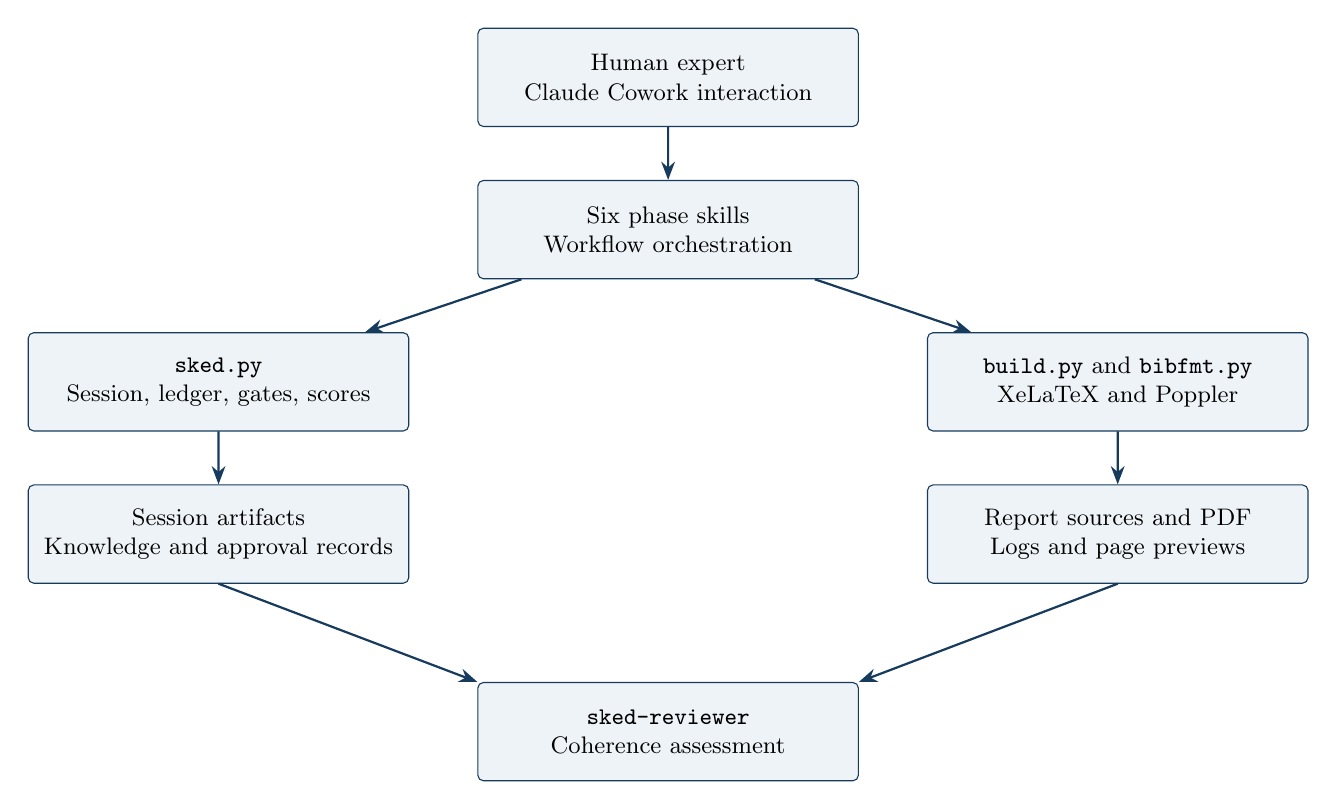
\begin{tikzpicture}[scale=0.96,transform shape,node distance=7mm and 9mm,
 box/.style={draw=navy,fill=pale,rounded corners=2pt,align=center,text width=48mm,minimum height=13mm,font=\small},
 arr/.style={-{Stealth},draw=navy,thick}]
\node[box] (human) {Human expert\\Claude Cowork interaction};
\node[box,below=of human] (skills) {Six phase skills\\Workflow orchestration};
\node[box,below left=of skills] (engine) {\texttt{sked.py}\\Session, ledger, gates, scores};
\node[box,below right=of skills] (build) {\texttt{build.py} and \texttt{bibfmt.py}\\XeLaTeX and Poppler};
\node[box,below=of engine] (state) {Session artifacts\\Knowledge and approval records};
\node[box,below=of build] (pdf) {Report sources and PDF\\Logs and page previews};
\node[box,below=13mm of $(state.south)!0.5!(pdf.south)$] (review) {\texttt{sked-reviewer}\\Coherence assessment};
\draw[arr] (human)--(skills);
\draw[arr] (skills)--(engine);\draw[arr] (skills)--(build);
\draw[arr] (engine)--(state);\draw[arr] (build)--(pdf);
\draw[arr] (state.south)--(review.north west);\draw[arr] (pdf.south)--(review.north east);
\end{tikzpicture}
\caption{Principal SKED components and artifact dependencies. The reviewer reads the PDF and approved knowledge, without the dialogue under the prescribed review procedure.}
\label{fig:architecture}
\end{figure}

\subsection{Skills and reviewer}
\begingroup\small
\begin{longtable}{@{}P{35mm}P{23mm}P{101mm}@{}}
\toprule
Component & Phase & Responsibility\\
\midrule\endhead
\code{sked-start} & 1 and routing & Suitability, session creation, context packet, initial frame, and continuation routing.\\
\code{sked-dialogue} & 2 & Question selection, interpretation, ledger operations, round closure, and stopping decisions.\\
\code{sked-synthesis} & 3 & Resolve proposals and conflicts, verify sources, write and obtain approval of the consensus.\\
\code{sked-structure} & 4 & Plan sections and artifacts, associate entries with sections, check coverage, and obtain approval.\\
\code{sked-latex} & 5 & Scaffold, write sources, build, inspect pages, invoke quality assessment, and deliver.\\
\code{sked-quality} & 5 & Check coverage, coordinate coherence review, judge formal criteria, and compute acceptance.\\
\code{sked-reviewer} & Review role & Identify contradictions, unsupported content, terminology problems, and logical gaps against the PDF and consensus.\\
\bottomrule
\end{longtable}
\endgroup

The reviewer agent is instructed to use fresh context and not receive the dialogue. This provides a different reading task, but it is not an external human review or proof of statistical independence. If a separate agent cannot be used, the quality skill prescribes self-review and disclosure that the review was not independent. The reviewer should report issues without rewriting the document.

\subsection{Executable utilities}
The session engine \code{sked.py} owns session creation, event operations, state reconstruction, convergence, exports, file confirmations, coverage, scaffolding, and quality scoring. It uses the Python standard library. Its \code{Session} class reads the session metadata and logs, and writes metadata through a temporary file followed by replacement.

The build utility \code{build.py} checks or installs selected dependencies when requested, renders the bibliography, invokes XeLaTeX, analyzes logs, examines PDF metadata and fonts, and generates page previews. It imports \code{bibfmt.py}, which parses BibTeX-like input and renders references for the selected profile. Optional Pillow support produces contact sheets from the individual page images.

The class \code{skedreport.cls} defines report typography, headings, localized labels, title material, captions, citations, appendix behavior, and invisible ledger tags. The template \code{main.tex} is populated with metadata during scaffolding. The documentation itself is a separate self-contained LaTeX file and does not require this custom class.

\subsection{Execution and persistence boundary}
Claude orchestrates the work. The scripts do not autonomously ask questions, call a model API, search the web, or decide whether an expert has genuinely consented. Commands can be called directly outside the intended dialogue. Accordingly, phase checks constrain script-mediated transitions but are not a complete authorization or policy-enforcement boundary.

State is stored as ordinary files in the selected workspace. Preservation across Cowork tasks depends on retaining that folder and making it accessible again. Plugin installation and session persistence are separate concerns. Updating the installed plugin does not by itself migrate session data or prove compatibility with older generated class files.
\source{scripts/sked.py; scripts/build.py; scripts/bibfmt.py; agents/sked-reviewer.md}

\section{Session artifacts and knowledge representation}
\subsection{Directory structure}
\begin{Code}
sked-sessions/<slug>/
  session.json
  ledger.jsonl
  dialogue.jsonl
  kstar.md
  structure.md
  report/
    main.tex
    skedreport.cls
    refs.bib
    references.tex
    sections/
    figures/
    main.pdf
    build/
      build-summary.json
      preview/
  quality/
    coherence.json
    fc-judged.json
    quality.json
    quality.md
\end{Code}
The session slug is derived from the topic or supplied explicitly. Initialization refuses to replace an existing \code{session.json} at the selected location. Metadata includes the plugin version, topic, timestamps, phase, next round, mode, languages, parameters, context, metrics, approvals, and recorded convergence.

\code{ledger.jsonl} stores knowledge events. \code{dialogue.jsonl} stores compact exchanges and move labels. The latter is not guaranteed to be a verbatim transcript. The consensus and outline are human-readable Markdown artifacts. The report directory contains both editable sources and derived output. Quality artifacts preserve the structured assessments used by the score.

\subsection{Entries and provenance}
Entry identifiers use \code{K} for knowledge, \code{Q} for questions, and \code{S} for sources, followed by an integer. The knowledge types are claim, definition, assumption, constraint, decision, requirement, and example. Questions and sources are additional entry types.

\begin{longtable}{@{}P{30mm}P{129mm}@{}}
\toprule
Field & Meaning and supported values\\
\midrule\endhead
\code{id}, \code{type} & Stable entry identifier and one of the supported categories.\\
\code{text} & An atomic statement or question, normally in the document language.\\
\code{origin} & \code{H} for human, \code{M} for model, or \code{S} for external-source content.\\
\code{status} & \code{proposed}, \code{agreed}, \code{contested}, \code{open}, \code{deferred}, \code{resolved}, or \code{retracted}.\\
\code{priority} & \code{high}, \code{normal}, or \code{low}. Coverage weights are 3, 2, and 1.\\
\code{verified} & \code{none}, \code{human}, or \code{source}. This is a recorded assessment.\\
\code{refs} & Links to source identifiers associated with an entry.\\
\code{term}, \code{note} & Definition term and supplementary explanation.\\
\code{bib}, \code{bibkey} & Bibliographic input and citation key for a source entry.\\
\code{section} & An editable section association supported by the engine.\\
\bottomrule
\end{longtable}

For an ordinary new human-origin entry, the default status is agreed and verification is human. Model-origin contributions default to proposed and unverified. Questions default to open. Assigning agreed status to an unverified model entry marks it human-verified during replay. Source verification still requires an explicit source-level assessment.

The engine validates enumerated values on several operations, but it is not a comprehensive schema validator. Status values are not restricted to a type-specific transition graph. Some edit fields receive less validation than initial additions. Source links are not automatically dereferenced or evaluated for evidential support. Operational discipline remains necessary.

\subsection{Event operations and replay}
The supported operations are \code{add}, \code{edit}, \code{status}, \code{verify}, \code{retract}, and \code{turn}. Knowledge operations are appended to the ledger with timestamps and round numbers. Turn operations go into the dialogue log. Replay reconstructs entries in event order and retains revision information. Retracted entries are omitted from ordinary views but can be requested explicitly.

A batch can refer to an earlier addition through \code{$1}, \code{$2}, and similar placeholders. These count additions, not arbitrary operation positions. Forward references should not be used. The engine collects new events before appending them, but writes the ledger, dialogue, and metadata separately. There is no multi-file database transaction or session lock. Run one writer per session and preserve backups before manual recovery.

\subsection{Consensus export}
The exporter collects agreed or resolved knowledge entries, groups definitions and statements, lists open and deferred questions, and includes source records. It preserves a narrative between designated markers when regenerating the file. The skill asks Claude to write that narrative in approximately 120--300 words, using only ledger content.

The actual export may also list outstanding proposed or contested entries under an explicit exclusion heading. The confirmation command normally refuses outstanding non-source, non-question proposals or conflicts and rejects an unchanged narrative placeholder. It does not prove that the narrative is faithful or that all questions were resolved. Review the complete artifact before approval.
\source{references/ledger-schema.md; scripts/sked.py, Session, apply_ops, fold, build_kstar}

\section{Five phases and transition checks}
\subsection{Initialization}
Phase 1 creates the session and context, constructs the initial model frame $K^{(0)}$, and records the first question. Round zero is initialization rather than an elicitation round. Closing it records an initial metric and increments the next-round counter. Later phase transitions check that a metric for round zero exists.

A useful initial frame makes scope, assumptions, and unknowns visible. It must remain challengeable. The mode and context packet are stored configuration; the quality of the frame and the suitability of the first question are prescribed by the skills rather than computed by the engine.

\subsection{Socratic dialogue}
Phase 2 iterates through interpretation, knowledge extraction, next-move selection, event application, and round closure. Each answer can add, refine, contest, resolve, defer, or retract entries. Counterquestions from the human should be answered before Claude asks the next elicitation question.

Round closure records metrics and reports convergence readiness, budget exhaustion, and the model-proposal acceptance warning. It does not itself move to synthesis. The \code{converge} command records why elicitation ended, after which the phase command can enter phase 3. A numerical convergence request is rejected when criteria fail unless overridden. Human and budget stopping modes can record unresolved reasons.

\subsection{Synthesis}
Phase 3 resolves pending model proposals and contested knowledge, evaluates remaining questions, and verifies factual claims and bibliography records as prescribed. Unanswered model proposals should not be silently accepted. An unresolved question can be deferred, but its limitation must remain visible.

Claude writes the consensus narrative, shows it to the expert, and records approval only after the expert agrees. Confirmation saves the file hash, timestamp, and round. There is no separate authenticated human signature. A later phase check validates file identity against this saved hash.

\subsection{Structuring}
Phase 4 turns the approved knowledge into an outline and plans informative artifacts. The skill prescribes one primary section for each target entry and full plan coverage. Entries that have no meaningful section should trigger reconsideration of the outline or scope.

The plan coverage utility recognizes entry identifiers appearing anywhere in the Markdown file. It does not parse primary-section assignments, prove uniqueness, or determine whether a section adequately represents an entry. Moreover, \code{confirm structure} does not automatically run coverage. Full mapping is therefore a prescribed step that must be performed and reviewed before confirmation.

\subsection{Production and acceptance}
Phase 5 scaffolds the report, generates sections from the approved knowledge and outline, produces planned artifacts, compiles, inspects pages, and assesses quality. New knowledge discovered during writing should return to the ledger and approval workflow. It should not be inserted directly as an untracked factual addition.

The transition to \code{done} checks prior approvals and the stored quality result. The intended workflow rebuilds and recomputes that result immediately before delivery. The engine does not automatically establish that the stored result is newer than every edited source file.

\subsection{What transition checks guarantee}
\begin{longtable}{@{}P{32mm}P{127mm}@{}}
\toprule
Requested target & Normal programmatic prerequisites\\
\midrule\endhead
Phase 2 & A closed round zero.\\
Phase 3 & Closed round zero and a recorded convergence decision.\\
Phase 4 & The preceding conditions and an existing consensus file matching its confirmation hash.\\
Phase 5 & The preceding conditions and an existing outline matching its confirmation hash.\\
\code{done} & The preceding conditions and a stored quality result with \code{passed} set to true.\\
\bottomrule
\end{longtable}
These checks are based on the requested target. The engine does not require adjacent transitions and does not block every command that would be inappropriate in the current phase. The \code{--force} option bypasses checks where provided. The skills reserve it for an explicit human override, but that restriction is procedural. Avoid it during ordinary use.
\source{scripts/sked.py, cmd_round_close, cmd_converge, cmd_confirm, cmd_phase}

\section{Convergence and dialogue indicators}
\subsection{The state projection}
For an active ledger state, the implementation constructs
\begin{equation}
 A_t=\{(\mathrm{id}_i,\operatorname{norm}(\mathrm{text}_i),\mathrm{status}_i)\mid i\in\mathcal{E}_t\}.
\end{equation}
The symbols and set notation have the following meanings.
\begin{itemize}
\item $A_t$ is the set of projected active-entry tuples after all events through round $t$ have been replayed.
\item $t$ is the nonnegative integer round index. Round $0$ represents initialization.
\item $\mathcal{E}_t$ is the index set of all active ledger entries at round $t$, excluding retracted entries.
\item $i$ identifies one entry in $\mathcal{E}_t$; $\mathrm{id}_i$ is its stable ledger identifier, such as \code{K1}, \code{Q1}, or \code{S1}.
\item $\mathrm{text}_i$ is the stored text of entry $i$ at the selected round, and $\mathrm{status}_i$ is its status at that round. The round dependence of these fields is implicit to match the implementation-oriented notation.
\item $\operatorname{norm}(\cdot)$ is the text-normalization function described below; the centered dot denotes its argument.
\item Parentheses delimit an ordered tuple. Braces collect the tuples into a set. The vertical bar means ``such that'', and $i\in\mathcal{E}_t$ means that the tuples are formed for entries in the active index set.
\end{itemize}
Normalization applies Unicode NFC normalization, case folding, whitespace collapse, and trimming. Retracted entries are excluded. The resulting set includes active questions and sources as well as knowledge entries. Changes to priority, verification, references, or other metadata do not change this projection when text and status remain unchanged.

The round distance is
\begin{equation}
 \delta_t=1-\frac{|A_t\cap A_{t-1}|}{|A_t\cup A_{t-1}|},
\end{equation}
The symbols and operators have the following meanings.
\begin{itemize}
\item $\delta_t$ is the dimensionless Jaccard distance between the projected ledger states at rounds $t$ and $t-1$.
\item $t$ is the current closed-round index, and $t-1$ identifies the preceding round. For initialization, the implementation compares round $0$ with an empty prior state.
\item $A_t$ and $A_{t-1}$ are the current and preceding sets of active-entry tuples, respectively.
\item $\cap$ denotes set intersection, so $A_t\cap A_{t-1}$ contains tuples unchanged between the two states.
\item $\cup$ denotes set union, so $A_t\cup A_{t-1}$ contains every distinct tuple present in either state.
\item $|B|$ denotes the cardinality, or number of elements, of a set $B$; $B$ is a generic set used here to explain the notation. The constant $1$ converts Jaccard similarity into distance.
\end{itemize}
The implementation returns $\delta_t=0$ when both sets are empty, avoiding a zero denominator. The distance lies between zero and one on the projected sets. It is not a distance that distinguishes all possible full ledger states, because different metadata can map to the same projection.

\subsection{Interpretation and an example}
If ten entry tuples remain unchanged and one is added, the distance is $1/11$, approximately $0.091$. If the text of one among ten entries is replaced, the union contains eleven tuples and the intersection nine, giving approximately $0.182$. The indicator treats the replacement as removal of an old tuple and addition of a new one. It does not measure semantic similarity between the two formulations.

A priority-only change can yield zero distance. Conversely, a small textual revision may create a substantial distance in a short ledger. A large stable ledger can dilute the effect of a new important entry. These consequences follow from the chosen projection and denominator. They should guide interpretation of the dashboard rather than be hidden behind the word convergence.

\subsection{Default stopping conditions}
Automatic readiness requires at least three closed dialogue rounds excluding round zero, two consecutive stored distances strictly below $0.05$, no open high-priority question, and no contested entry. The engine stores the distances rounded to four decimal places, and readiness uses those stored values. The maximum-round budget is fifteen dialogue rounds by default. Reaching it asks for a human decision under the skill policy rather than automatically proving agreement.

Pending model proposals are reported separately and do not directly block the numerical readiness calculation. They must still be resolved during synthesis before ordinary consensus confirmation. Open questions of normal or low priority may also remain. The human's decision can end elicitation even if the numerical conditions are not satisfied, provided that the unresolved matters are handled explicitly.

\subsection{Model-proposal acceptance warning}
The engine counts model-origin non-source, non-question entries whose final status is agreed, retracted, or contested. It reports how many were agreed without an edit. A ratio above $0.8$ across at least five such decisions triggers a warning. The prescribed response is to ask more open questions and invite the expert to restate important positions.

This indicator is a prompt to reconsider the dialogue. It does not diagnose sycophancy or determine whether the accepted proposals were correct. A knowledgeable expert can legitimately accept several correct proposals unchanged. The warning is not a hard transition blocker.
\source{scripts/sked.py, norm, state_set, jaccard_distance, convergence, m_acceptance}

\section{Document quality and acceptance}
\subsection{Composite score}
The configurable score and its default coefficients are
\begin{equation}
 Q(R)=\alpha C_q+\beta C_{\mathrm{oh}}+\gamma F_c
      =0.4C_q+0.3C_{\mathrm{oh}}+0.3F_c,
\end{equation}
The symbols and coefficients have the following meanings.
\begin{itemize}
\item $R$ is the document being assessed, and $Q(R)$ is its dimensionless composite acceptance score.
\item $C_q$ is the dimensionless, priority-weighted coverage of target knowledge entries. The subscript $q$ is the package's coverage-component label, not a summation index.
\item $C_{\mathrm{oh}}$ is the dimensionless coherence score derived from the review. The subscript $\mathrm{oh}$ is a descriptive component label; together with $C$ it corresponds to the package's \code{Coh} notation.
\item $F_c$ is the dimensionless formal-compliance score, defined as the fraction of included checks that pass. The subscript $c$ labels compliance and is not the critical-issue index used later in $n_c$.
\item $\alpha$, $\beta$, and $\gamma$ are dimensionless weights assigned to coverage, coherence, and formal compliance, respectively. Their defaults are $0.4$, $0.3$, and $0.3$; their intended constraints are nonnegativity and $\alpha+\beta+\gamma=1$.
\end{itemize}
The default acceptance threshold is $0.85$. With component values in $[0,1]$ and the intended weight constraints, $Q(R)$ also lies in $[0,1]$. The score is an internal workflow criterion. No calibration study, measurement uncertainty, inter-rater reliability estimate, or comparison benchmark is provided in the archive.

Weights and thresholds are configurable. The setter accepts many values without comprehensive numerical validation. Keep nonnegative weights summing to one if the score is to retain its intended interpretation. A higher threshold does not repair weak evidence or incomplete checklists.

\subsection{Tagged knowledge coverage}
The target set contains agreed or resolved knowledge entries and deferred questions. Each target has weight three, two, or one for high, normal, or low priority. Coverage is
\begin{equation}
 C_q=\frac{\sum_{i\in\mathcal{T}}w_i I_i}{\sum_{i\in\mathcal{T}}w_i},
\end{equation}
The symbols and operators have the following meanings.
\begin{itemize}
\item $C_q$ is the dimensionless weighted coverage score for the outline or report under inspection.
\item $\mathcal{T}$ is the target set of agreed or resolved knowledge entries and deferred questions that should be represented.
\item $i$ indexes a target entry, and $i\in\mathcal{T}$ indicates that the sums range over that target set.
\item $w_i$ is the positive, dimensionless priority weight of entry $i$, equal to $3$, $2$, or $1$ for high, normal, or low priority, respectively.
\item $I_i$ is a binary coverage indicator. It equals $1$ when the entry identifier is detected in the inspected outline or report tags and equals $0$ otherwise.
\item $\sum$ denotes summation over the indicated target entries. The numerator is the total covered weight, and the denominator is the total target weight.
\end{itemize}
For a nonempty target set, $C_q$ lies in $[0,1]$. An empty target set produces coverage one by implementation convention. This is a degenerate condition, not evidence of a complete technical report.

For an outline, identifiers are detected in Markdown. For a report, the engine scans LaTeX files recursively, excluding directories named \code{build} and files named \code{references.tex}, and extracts \verb|\sked{...}| tags. The tags are invisible in the ordinary PDF. A review build exposes them for inspection.

The scan is lexical. It is not restricted to the exact transitive input graph of the compiled document, so an unused LaTeX file in the report tree can contribute tags. A tag does not prove that surrounding prose expresses the entry. Untagged claims can escape coverage accounting entirely. The quality skill therefore requests spot checks, and the reviewer compares document content with the approved knowledge.

\subsection{Coherence assessment}
The reviewer examines contradictions, distortion of the consensus, unsupported claims, inconsistent terminology, logical gaps, unsupported abstracts or conclusions, and deferred matters presented as settled. Issues are classified as critical, major, or minor. The default calculation is
\begin{equation}
 C_{\mathrm{oh}}=\max(0,1-0.15n_c-0.07n_m-0.02n_l),
\end{equation}
The symbols, constants, and operator have the following meanings.
\begin{itemize}
\item $C_{\mathrm{oh}}$ is the dimensionless coherence score for the assessed document.
\item $n_c$ is the nonnegative integer count of critical issues; the subscript $c$ denotes critical severity.
\item $n_m$ is the nonnegative integer count of major issues; the subscript $m$ denotes major severity.
\item $n_l$ is the nonnegative integer count of minor issues; the subscript $l$ denotes minor severity.
\item $0.15$, $0.07$, and $0.02$ are the dimensionless penalties per critical, major, and minor issue, respectively.
\item The constant $1$ is the score assigned when no issues are recorded. The constant $0$ is the lower bound.
\item $\max(a,b)$ returns the larger of its two arguments $a$ and $b$; these letters are generic operator arguments, not additional document parameters. Here the operator prevents accumulated penalties from producing a negative score.
\end{itemize}
Under this penalty rule, $C_{\mathrm{oh}}$ lies in $[0,1]$. The assessment is stored in \code{quality/coherence.json}. Missing review is a blocker.

The reviewer instructions say to omit a numerical score because the engine computes it. The implementation nevertheless accepts an explicit \code{score} field if one is supplied. For reproducible use of the documented penalty rule, omit that field and preserve the issue records. Coherence depends on reviewer sensitivity and issue granularity, so scores are not directly comparable across reviewers without a controlled protocol.

\subsection{Formal compliance}
Formal checks combine automatic records and optional human- or model-judged items. Automatic checks inspect compilation, undefined references and citations, excessive overfull boxes, missing glyphs, hyphenation, font embedding, bibliography consistency, source verification labels, float references, placeholders, selected style rules, and use of entries in inappropriate states. Judged items address title material, abstract, keywords, section order, captions, terminology, page layout, limitations, and profile-specific requirements.

The formal component is the count of passed items divided by the number of included items. Checks have equal weight. Adding or omitting judged items changes both the numerator and denominator. The scoring function does not require a complete judged checklist to exist. Follow the profile checklist and retain every result rather than selecting only easy passes.

Several checks are heuristics. Source verification is based on stored labels, not a fresh source retrieval. The numeric-claim detector looks for a digit in a tagged model-origin entry and does not understand the meaning of the number. Static reference and style checks use regular expressions rather than a complete TeX parser.

\subsection{Hard blockers and procedural failures}
The implemented hard blockers are an absent or unsuccessful build, uncovered high-priority targets, tagged model-origin claims containing digits without source verification, critical coherence issues, missing coherence review, and cited keys missing from the bibliography build result. Acceptance requires meeting the score threshold with none of these blockers.

Other failed formal items can coexist with a passing composite score. Thus a programmatic pass is weaker than the skill's prescribed procedure, which asks Claude to fix failed checks and inspect rendered pages. The build utility's successful exit also means less than final acceptance. It indicates production of a PDF without recorded LaTeX errors, not satisfaction of every layout or factual requirement.

The quality instructions allow at most three repair loops by default before remaining issues are presented to the user. This limit is stored as a parameter but is not an autonomous loop enforced by the scoring function. The model follows it as a workflow instruction.
\source{scripts/sked.py, coverage, static_tex_checks, quality; skills/sked-quality/SKILL.md}

\section{LaTeX production and bibliography pipeline}
\subsection{Scaffolding and content generation}
Scaffolding creates the report, sections, and figures directories, copies the report class, renders the initial metadata into \code{main.tex}, and writes bibliography input from ledger source entries. Existing \code{main.tex} is retained unless forced. The class is copied and the bibliography is regenerated during scaffolding, so back up intentional local modifications before repeating it.

Claude writes one source file per major section and adds the relevant input statements. Knowledge-bearing paragraphs, lists, captions, and table notes should carry ledger tags. New claims require ledger handling and approval. Abstract and conclusions should summarize supported content rather than introduce additional results.

The class supports metadata commands, localized cross-references, figures, tables, algorithms, Unicode-safe code listings, and appendices. Figure labels and arrow routes should be checked visually. For Cyrillic code, the package prescribes its \code{skedcode} environment rather than relying on ASCII-oriented listing behavior under XeTeX.

\subsection{Profiles and their scope}
\begin{longtable}{@{}P{22mm}P{137mm}@{}}
\toprule
Profile & Implemented intent and main defaults\\
\midrule\endhead
\code{ieee} & A technical-report layout with numeric references, A4, 11 pt text, side margins of 25 mm, and top and bottom margins of 27 mm. It is not an official journal-specific IEEE template.\\
\code{dstu} & A Ukrainian research-report layout with 14 pt text, 1.5 spacing, and left/right/top/bottom margins of 25/15/20/20 mm. References use a simplified DSTU-oriented formatter. Institutional requirements still need checking.\\
\code{apa} & An APA-oriented report layout with A4 paper, 12 pt text, double spacing, 25.4 mm margins, and author-year references. Exact publication compliance requires review.\\
\bottomrule
\end{longtable}
The engine localizes its generated consensus text for Ukrainian and English. The class and build utility recognize additional language names in selected places, but their presence does not establish complete localization or tested multilingual support. Fonts are selected from an availability-ordered list that prefers Times New Roman and then alternatives including Liberation Serif.

\subsection{Bibliography rendering}
The Python formatter reads \code{refs.bib}, follows supported citation and input patterns, orders references, creates \code{references.tex}, and reports missing keys, uncited entries, and incomplete records. Numeric profiles default to citation order; the APA path uses author-oriented ordering. An explicit bibliography order can also be requested.

This removes the normal dependency on an external BibTeX or biber run for this pipeline. It is a custom parser and renderer rather than a complete implementation of every BibTeX construct or every style rule. Verify names, transliteration, punctuation, dates, URLs, and the rendered entries against the target venue. A plausible reference format does not verify that a publication exists or supports the cited statement.

The package README suggests that delivered sources compile anywhere with two XeLaTeX runs. The executable build path generates \code{references.tex} first and may perform additional runs for settled references. Portable delivery therefore requires the generated bibliography file or access to the formatter, the report class, appropriate fonts, and required TeX packages.

\subsection{Build and inspection}
The build command optionally checks dependencies, renders references, invokes XeLaTeX at least twice under its normal default run limit, and repeats when the log indicates another run is needed, up to the configured maximum. It records errors, unresolved references, citations, overfull boxes, glyph issues, font warnings, hyphenation information, and PDF metadata in \code{build-summary.json}.

Poppler tools supply page information, font checks, and PNG previews. Pillow can assemble contact sheets. Generating previews does not mean that they were viewed. The skill explicitly requests inspection of all pages through thumbnails and full-size inspection of the title page and pages containing complex artifacts.

The \code{--ensure-deps} option can invoke \code{apt-get} when the process is root and that package manager is available. This is an environment-modifying operation, not a portable installation mechanism. It may be unavailable in Cowork or constrained by package repositories and network policy. Missing dependencies should be reported accurately rather than hidden behind repeated build attempts.
\source{scripts/build.py; scripts/bibfmt.py; templates/skedreport.cls; references/latex-guide.md}

\section{Command and configuration reference}
\subsection{Execution convention}
Ordinary users interact with Claude in natural language. The commands below are for maintainers, diagnosis, and explaining what Claude executes. Replace the plugin path and session directory with actual paths in the Cowork execution environment. The examples use shell variables only as readable local aliases.
\begin{Code}
SKED_PLUGIN_DIR=/actual/path/to/sked
SKED_SESSION_DIR=/actual/work/sked-sessions/example
python3 "$SKED_PLUGIN_DIR/scripts/sked.py" \
  --session "$SKED_SESSION_DIR" status
\end{Code}
The global \code{--session} option precedes the subcommand. Session discovery checks the explicit argument, then \code{SKED_SESSION}, then the current directory, then a single session beneath \code{./sked-sessions}. Multiple matches require an explicit choice.

\subsection{Session commands}
\begin{longtable}{@{}P{47mm}P{112mm}@{}}
\toprule
Command & Purpose and important options\\
\midrule\endhead
\code{init} & Requires \code{--topic}. Options include \code{--root}, \code{--slug}, \code{--profile}, \code{--mode}, \code{--lang-dialogue}, and \code{--lang-doc}. Defaults are IEEE, deep mode, and Ukrainian languages.\\
\code{list} & Lists sessions beneath \code{--root}.\\
\code{set KEY VALUE} & Sets a dotted metadata path. Attempts JSON parsing of the value and otherwise stores a string.\\
\code{apply FILE} & Applies event operations from a file, or from standard input when the file argument is a hyphen.\\
\code{round-close} & Stores current-round metrics and advances the round. Supports \code{--note} and \code{--json}.\\
\code{show} & Filters entries by type, status, origin, identifier, or round. \code{--all} includes retracted entries. Output can be Markdown or JSON.\\
\code{dialogue} & Shows saved exchanges, optionally limited with \code{--last}. Supports JSON output.\\
\code{status} & Displays phase, counts, metrics, unresolved conditions, approvals, and the next suggested step.\\
\code{converge} & Requires \code{--by delta}, \code{human}, or \code{budget}. Records stopping reasons and an optional note.\\
\code{phase N} & Requests phase 1--5 or \code{done}, subject to target prerequisites unless forced.\\
\code{kstar} & Exports the consensus file and preserves its narrative block. Supports an alternate output path.\\
\code{confirm kstar} & Records the consensus file hash after normal proposal and placeholder checks.\\
\code{confirm structure} & Records the outline file hash. Does not itself validate plan coverage.\\
\code{coverage} & Scans the report or a file supplied through \code{--plan}. Supports JSON output.\\
\code{scaffold} & Creates report sources and writes class and bibliography files. \code{--force} can replace the main file.\\
\code{bib} & Rewrites bibliography input from ledger source entries.\\
\code{quality} & Computes and writes the composite assessment for the selected report directory.\\
\bottomrule
\end{longtable}

\subsection{Default parameters}
\begin{longtable}{@{}P{58mm}P{23mm}P{78mm}@{}}
\toprule
Parameter & Default & Meaning\\
\midrule\endhead
\code{epsilon} & 0.05 & Strict upper bound for stable round distances.\\
\code{stable_rounds} & 2 & Required consecutive stable rounds.\\
\code{min_rounds} & 3 & Minimum closed dialogue rounds.\\
\code{max_rounds} & 15 & Budget notification point.\\
\code{weights.alpha} & 0.4 & Tagged knowledge coverage weight.\\
\code{weights.beta} & 0.3 & Coherence weight.\\
\code{weights.gamma} & 0.3 & Formal compliance weight.\\
\code{q_threshold} & 0.85 & Composite acceptance threshold.\\
\code{overfull_tolerance_pt} & 1.0 & Quality-check tolerance for reported overfull boxes.\\
\code{max_fix_loops} & 3 & Prescribed maximum repair loops before reporting remaining issues.\\
\bottomrule
\end{longtable}
These values are stored under \code{params}. For example, changing \code{params.epsilon} changes the intended convergence threshold. Such changes should reflect the task and be documented before assessment, rather than made only to obtain a pass. Context and house-style rules are separate fields under \code{context}.

\subsection{Build commands}
\begin{Code}
python3 "$SKED_PLUGIN_DIR/scripts/build.py" \
  --dir "$SKED_SESSION_DIR/report"

python3 "$SKED_PLUGIN_DIR/scripts/build.py" \
  --dir "$SKED_SESSION_DIR/report" --review

python3 "$SKED_PLUGIN_DIR/scripts/sked.py" \
  --session "$SKED_SESSION_DIR" coverage --json

python3 "$SKED_PLUGIN_DIR/scripts/sked.py" \
  --session "$SKED_SESSION_DIR" quality
\end{Code}
Additional build options include \code{--ensure-deps}, \code{--no-previews}, \code{--dpi}, \code{--max-runs}, \code{--bib-order}, \code{--main}, and \code{--update-class}. Replacing a customized class with \code{--update-class} should be intentional. The standalone bibliography utility also exposes command help for formatter-specific use.

\section{Illustrative workflow}
\subsection{Scenario and initialization}
This example is a recommended teaching scenario, not a measured Cowork case study. Suppose a research engineer wants to document an internal dataset-cleaning procedure. The desired output is an English report that another engineer can reproduce. The expert knows the processing steps but has not yet separated requirements, assumptions, and observed outcomes.

Claude collects the intended reader, example inputs, available measurements, and exclusions. The initial model frame proposes that the report should cover input validation, duplicate handling, missing-value policy, output artifacts, and limitations. Those are proposed areas for discussion rather than claims that the procedure actually implements them.

\subsection{Elicitation and ledger changes}
The expert explains that duplicate records are detected by a normalized identifier, while near-duplicates are outside scope. Claude should record the first statement as a claim and the second as a constraint. If the expert says the procedure is probably faster than an earlier version, the statement remains a proposal or assumption until supporting evidence exists.

A minimal illustrative event batch might be
\begin{Code}
[
  {"op":"add", "type":"claim", "origin":"H",
   "text":"Exact duplicates are detected by normalized identifier.",
   "priority":"high"},
  {"op":"add", "type":"constraint", "origin":"H",
   "text":"Near-duplicate detection is outside the procedure scope."},
  {"op":"add", "type":"question", "origin":"M",
   "text":"What evidence supports a performance improvement?",
   "priority":"normal"}
]
\end{Code}
The human-origin defaults record agreement and human verification. That is appropriate for describing the expert's own procedure, but it does not independently establish implementation correctness. If the performance question cannot be answered, it can be deferred and later presented as a limitation.

\subsection{Consensus and structure}
After the dialogue is ended and recorded, Claude resolves outstanding proposals, exports the consensus, and writes a short narrative that preserves the distinction between supported behavior and unmeasured performance. The expert approves the content. The outline then assigns each entry to a primary section and plans a process diagram, a table of input assumptions, and a reproducibility checklist.

A sound coverage review asks whether each section actually explains its associated entries. Merely putting every identifier into a list would satisfy the lexical plan scan but defeat its purpose. Approval should follow this substantive review.

\subsection{Production and delivery}
Claude writes section files, marks knowledge-bearing material with ledger tags, and creates the diagram and tables. The build produces a PDF and diagnostics. The reviewer checks the PDF against the consensus, including whether the abstract accidentally claims a measured speed improvement. Formal review checks captions, page layout, citations, and stated limitations.

The final delivery includes the compiled report and, when requested, the source files. The limitation concerning performance remains explicit. No benchmark numbers or quality scores are supplied in this example because none were measured. A later experiment should enter through new ledger evidence, followed by the relevant approvals and rebuild.

\section{Limitations and assurance boundary}
\subsection{Knowledge and model limitations}
SKED cannot guarantee that an expert's statement is correct, that a model interpretation preserves every nuance, or that a retrieved source supports a claim. The ledger improves inspectability only when entries are atomic, attributed correctly, and reviewed. Incorrect agreement can be retained faithfully. A stable dialogue can also be incomplete if important questions were never asked.

Source verification is represented by a label and references. The engine does not automatically inspect remote evidence, reproduce experiments, or authenticate the reviewer. Its digit detector can miss quantities written as words and can flag an identifier or version that is not an empirical claim. Human and model responsibilities therefore remain central to factual reliability.

\subsection{Approval and state consistency}
File hashes detect changes to the approved files. They do not automatically detect changes to the live ledger after approval. Coverage is calculated from the live ledger, while generation is prescribed to use the approved consensus. If the ledger changes without regenerating that file, these bases can diverge. The required operational response is to regenerate and reapprove affected artifacts.

There is no complete state machine restricting every command to its intended phase. Nonadjacent phase requests are possible when their prerequisites exist. Confirmation and override commands are callable by the same process that writes the files. This design supports an assisted workflow, not an independently authenticated approval system.

\subsection{Coverage and quality limitations}
Tagged coverage can be inflated by irrelevant tags or unused source files. Untagged additions can escape the accounting. Plan coverage does not establish one-to-one assignment or semantic adequacy. Reviewer findings depend on the reviewer, and a numerically high score can coexist with failed nonblocking checks.

Quality output and build summaries have no comprehensive freshness linkage to all inputs. The transition to done reads a stored pass. Always rebuild, review, and recalculate after relevant changes. The score should not be presented as a publication-readiness probability, a truth score, or a validated scientific measure.

\subsection{Persistence, compatibility, and portability}
Session files have no database-level concurrency protection or transactional update across all artifacts. Direct edits to the ledger can destroy replay validity. No explicit migration mechanism is included for future schema changes. Keep the inspected plugin version with archived sessions where reproducibility matters.

The README specifies Python 3.8 or later. The targeted execution checks for this manual used Python 3.12.14, not a supported-version matrix. Compatibility with every advertised Python version has not been established by those checks. Test the actual deployment interpreter and its dependencies before production use.

Cowork compatibility depends on installation, file access, Python execution, tool availability, and typesetting dependencies. No complete installation or interactive session was run in Cowork for this edition. Host operating-system paths should not be confused with paths inside the execution environment. A profile name does not establish exact compliance with a journal's submission template.

\subsection{Data handling and scope of protection}
The ledger, dialogue summaries, and reports may contain the expert's substantive knowledge. The package provides no encryption, access-control layer, secret redaction, or retention policy for these artifacts. Apply the host environment's file permissions and the organization's data-handling requirements. Local file storage alone does not imply that interactions with a hosted model remain entirely local.

The scripts and templates do not constitute a hardened sandbox for untrusted LaTeX or arbitrary external files. The appropriate operational boundary is a controlled working folder with reviewed source material. This statement describes absent mechanisms rather than an evaluated security vulnerability.
\source{scripts/sked.py; scripts/build.py; README.md; references/sked-method.md}

\section{Troubleshooting and recovery}
\begin{longtable}{@{}P{43mm}P{116mm}@{}}
\toprule
Observed condition & Diagnosis and recommended action\\
\midrule\endhead
Plugin is installed but no session starts & Confirm that SKED is available in the current Cowork task, that its resources can be located, and that the task can write to the chosen folder. Use an explicit start request.\\
Several sessions are reported & Identify the intended session and use its explicit directory. Do not let a new task silently select a different project.\\
Transition to synthesis fails & Inspect round zero and the convergence record. Numerical readiness must be explicitly recorded through the stopping command.\\
Consensus confirmation fails & Resolve pending proposals or contested entries and replace the narrative placeholder. Do not force approval merely to proceed.\\
Approved file changed & Review the new content and confirm it again. A new hash is expected after an intentional change.\\
Ledger changed after approval & Regenerate the consensus, review and approve it, and revise the outline and report where needed. File-hash checks alone do not perform this reconciliation.\\
XeLaTeX or packages missing & Check the execution environment. Use dependency installation only where supported and permitted. Report missing components when installation is unavailable.\\
Undefined citation or missing bibliography key & Correct the ledger source record and citation key, regenerate bibliography input, and rebuild. Do not edit only the derived reference file.\\
Overfull boxes or missing glyphs & Inspect the reported location and rendered page. Reword long tokens, adjust tables or diagrams, and choose fonts with the required characters.\\
Quality result is stale & Rebuild after edits, repeat relevant page inspection and review, then recalculate quality before marking the session done.\\
Malformed ledger JSON & Preserve a backup first. Locate the invalid line and restore from a known valid version. Avoid silently deleting history to obtain a successful replay.\\
\bottomrule
\end{longtable}

A reliable archive contains the complete session directory, the exact plugin version, and the final report sources. For lightweight source delivery, omit temporary build files but retain \code{references.tex}, the report class, section files, bibliography input, and external figures. Record dependency versions if future reproduction is important. Changes to the build environment may alter line breaks, pagination, fonts, and warnings even when source text is unchanged.

\section{Verification performed for this edition}
\subsection{Inspection scope}
The documentation was prepared from the archive named on the title page. Its manifest, six skill instructions, reviewer instructions, five reference files, three Python scripts, and template interfaces were inspected. The executable source was used to qualify broader statements in the README, especially concerning gates, coverage, quality, and build portability.

The archive SHA-256 is given below to identify the inspected bytes.
\begin{Code}
8ba9cb85f453a283a550f16c922618e2998dcb04968b16ef8f41bf113f960ed6
\end{Code}
This identifies a source snapshot. It does not authenticate its publisher or establish that a future repository download will contain the same bytes.

\subsection{Targeted execution checks}
Selected mechanisms were exercised in a temporary local session without a Cowork client. The checks support narrow implementation statements rather than an overall performance or compatibility claim.
\begin{longtable}{@{}P{49mm}P{110mm}@{}}
\toprule
Check & Observed result and interpretation\\
\midrule\endhead
Priority-only ledger edit & The projected Jaccard distance was zero. Metadata changes are not represented by the state projection.\\
Outline containing only an entry ID & Reported plan coverage was 1.0 for a one-entry target set. Presence is checked lexically rather than semantically.\\
Two successive text edits & Replay returned the second text. Event order determines the reconstructed entry state.\\
Ledger edit after file approval & The unchanged consensus file still passed its saved hash check. Approval identity does not automatically bind to the current ledger.\\
\bottomrule
\end{longtable}

The manual's LaTeX source is compiled and its rendered pages are checked separately as an artifact-production step. That confirms the readability of this manual, not the successful completion of a SKED-generated report. No full dialogue, independent document review, comparative experiment, journal compliance assessment, or end-to-end Cowork installation test is claimed.

\subsection{Recommended acceptance exercise}
Before relying on a new deployment, conduct one short Cowork session with a known subject and explicit expected statements. Confirm installation and resource access, create a session, record a correction, defer a question, approve knowledge and structure, generate the PDF, inspect a ledger tag, and verify that edits trigger the intended review procedure. Retain the files and actual observations.

For a research publication, separate this operational acceptance exercise from a controlled evaluation of SKED itself. Such an evaluation would require defined tasks, a baseline, an assessment protocol, independent judgments where feasible, and recorded outcomes. The archive does not supply those results, and this manual does not invent them.

\appendix
\section{Source traceability}
\begin{longtable}{@{}P{68mm}P{91mm}@{}}
\toprule
Package resource & Documentation basis\\
\midrule\endhead
\code{.claude-plugin/plugin.json} & Identity, version, author, and declared purpose.\\
\code{README.md} & Workflow summary, operational definitions, profiles, dependencies, and claimed differences from the unavailable report.\\
\code{references/sked-method.md} & Conceptual model, Socratic components, context packet, phases, indicators, and stated limitations.\\
\code{references/ledger-schema.md} & Session files, fields, operations, and command summary.\\
\code{references/socratic-moves.md} & Question priorities, dialogue patterns, extraction rules, and anti-patterns.\\
\code{references/style-profiles.md} & Presentation profiles and judged formal checklist.\\
\code{references/latex-guide.md} & Class interface, ledger tags, artifacts, and rendering procedure.\\
\code{skills/*/SKILL.md} & Prescribed phase behavior, approvals, review, revisions, and delivery.\\
\code{agents/sked-reviewer.md} & Coherence-review scope, severity definitions, and issue format.\\
\code{scripts/sked.py} & Executable session behavior, metrics, gates, coverage, and quality.\\
\code{scripts/build.py} & Dependencies, compilation, diagnostics, and previews.\\
\code{scripts/bibfmt.py} & Bibliography parsing and rendering.\\
\code{templates/skedreport.cls} & Layout, localization, tags, captions, and report interfaces.\\
\code{templates/main.tex} & Scaffold substitutions and initial report structure.\\
\bottomrule
\end{longtable}

\section{Reference material and document maintenance}
\begin{enumerate}
\item Kharchenko, K. SKED plugin, version 0.1.0. Source package \code{Sked-0.1.0-v1.zip}. Repository consulted on 29 October 2026. \url{https://github.com/konst1970/SKED}.
\item Anthropic. \emph{Use plugins in Claude}. Official Help Center. Consulted on 29 October 2026 for the general Cowork plugin interface and custom-file upload. \url{https://support.claude.com/en/articles/13837440-use-plugins-in-claude}.
\end{enumerate}
The second source is used only for the brief host-interface guidance. All SKED-specific claims derive from the inspected archive. No independent scholarly bibliography was supplied with this documentation request. The unavailable SKED v1.0.0 technical report is mentioned only to explain a reference inside the package and is not treated as consulted evidence.

Future editions should update the archive identifier, plugin version, command behavior, client interface notes, observed compatibility results, and known limitations. If implementation changes invalidate a documented caveat, replace it with evidence from the new source and appropriate execution checks. Keep documentation versioning separate from plugin versioning.

\section{Terminology}
\begin{longtable}{@{}P{40mm}P{119mm}@{}}
\toprule
Term & Meaning in this manual\\
\midrule\endhead
Context packet & Stored audience, exemplars, constraints, rubric, and metadata used to guide a session.\\
Knowledge ledger & The append-only sequence of events from which the current knowledge entries are reconstructed.\\
Round & A recorded interaction unit whose closure stores metrics and advances the round counter.\\
Consensus $\K$ & The approved knowledge artifact used as the prescribed content basis for generation. Agreement does not imply truth.\\
Gate & A programmatic prerequisite check or, where explicitly stated, a prescribed human review step.\\
Coverage & Weighted presence of target identifiers in an outline or LaTeX tags.\\
Coherence & The review-based assessment of logical and terminological consistency and fidelity to the agreed knowledge.\\
Formal compliance & The fraction of included automatic and judged presentation checks that pass.\\
Profile & A bundled report layout and reference-rendering configuration.\\
Verification label & A stored value recording human or source assessment, rather than an automatic proof of correctness.\\
\bottomrule
\end{longtable}
\end{document}
